
\documentclass{article} % For LaTeX2e
\usepackage{iclr2025_conference,times}

\usepackage{graphicx}

% Optional math commands from https://github.com/goodfeli/dlbook_notation.
%%%%% NEW MATH DEFINITIONS %%%%%

\usepackage{amsmath,amsfonts,bm}

% Mark sections of captions for referring to divisions of figures
\newcommand{\figleft}{{\em (Left)}}
\newcommand{\figcenter}{{\em (Center)}}
\newcommand{\figright}{{\em (Right)}}
\newcommand{\figtop}{{\em (Top)}}
\newcommand{\figbottom}{{\em (Bottom)}}
\newcommand{\captiona}{{\em (a)}}
\newcommand{\captionb}{{\em (b)}}
\newcommand{\captionc}{{\em (c)}}
\newcommand{\captiond}{{\em (d)}}

% Highlight a newly defined term
\newcommand{\newterm}[1]{{\bf #1}}


% Figure reference, lower-case.
\def\figref#1{figure~\ref{#1}}
% Figure reference, capital. For start of sentence
\def\Figref#1{Figure~\ref{#1}}
\def\twofigref#1#2{figures \ref{#1} and \ref{#2}}
\def\quadfigref#1#2#3#4{figures \ref{#1}, \ref{#2}, \ref{#3} and \ref{#4}}
% Section reference, lower-case.
\def\secref#1{section~\ref{#1}}
% Section reference, capital.
\def\Secref#1{Section~\ref{#1}}
% Reference to two sections.
\def\twosecrefs#1#2{sections \ref{#1} and \ref{#2}}
% Reference to three sections.
\def\secrefs#1#2#3{sections \ref{#1}, \ref{#2} and \ref{#3}}
% Reference to an equation, lower-case.
\def\eqref#1{equation~\ref{#1}}
% Reference to an equation, upper case
\def\Eqref#1{Equation~\ref{#1}}
% A raw reference to an equation---avoid using if possible
\def\plaineqref#1{\ref{#1}}
% Reference to a chapter, lower-case.
\def\chapref#1{chapter~\ref{#1}}
% Reference to an equation, upper case.
\def\Chapref#1{Chapter~\ref{#1}}
% Reference to a range of chapters
\def\rangechapref#1#2{chapters\ref{#1}--\ref{#2}}
% Reference to an algorithm, lower-case.
\def\algref#1{algorithm~\ref{#1}}
% Reference to an algorithm, upper case.
\def\Algref#1{Algorithm~\ref{#1}}
\def\twoalgref#1#2{algorithms \ref{#1} and \ref{#2}}
\def\Twoalgref#1#2{Algorithms \ref{#1} and \ref{#2}}
% Reference to a part, lower case
\def\partref#1{part~\ref{#1}}
% Reference to a part, upper case
\def\Partref#1{Part~\ref{#1}}
\def\twopartref#1#2{parts \ref{#1} and \ref{#2}}

\def\ceil#1{\lceil #1 \rceil}
\def\floor#1{\lfloor #1 \rfloor}
\def\1{\bm{1}}
\newcommand{\train}{\mathcal{D}}
\newcommand{\valid}{\mathcal{D_{\mathrm{valid}}}}
\newcommand{\test}{\mathcal{D_{\mathrm{test}}}}

\def\eps{{\epsilon}}


% Random variables
\def\reta{{\textnormal{$\eta$}}}
\def\ra{{\textnormal{a}}}
\def\rb{{\textnormal{b}}}
\def\rc{{\textnormal{c}}}
\def\rd{{\textnormal{d}}}
\def\re{{\textnormal{e}}}
\def\rf{{\textnormal{f}}}
\def\rg{{\textnormal{g}}}
\def\rh{{\textnormal{h}}}
\def\ri{{\textnormal{i}}}
\def\rj{{\textnormal{j}}}
\def\rk{{\textnormal{k}}}
\def\rl{{\textnormal{l}}}
% rm is already a command, just don't name any random variables m
\def\rn{{\textnormal{n}}}
\def\ro{{\textnormal{o}}}
\def\rp{{\textnormal{p}}}
\def\rq{{\textnormal{q}}}
\def\rr{{\textnormal{r}}}
\def\rs{{\textnormal{s}}}
\def\rt{{\textnormal{t}}}
\def\ru{{\textnormal{u}}}
\def\rv{{\textnormal{v}}}
\def\rw{{\textnormal{w}}}
\def\rx{{\textnormal{x}}}
\def\ry{{\textnormal{y}}}
\def\rz{{\textnormal{z}}}

% Random vectors
\def\rvepsilon{{\mathbf{\epsilon}}}
\def\rvtheta{{\mathbf{\theta}}}
\def\rva{{\mathbf{a}}}
\def\rvb{{\mathbf{b}}}
\def\rvc{{\mathbf{c}}}
\def\rvd{{\mathbf{d}}}
\def\rve{{\mathbf{e}}}
\def\rvf{{\mathbf{f}}}
\def\rvg{{\mathbf{g}}}
\def\rvh{{\mathbf{h}}}
\def\rvu{{\mathbf{i}}}
\def\rvj{{\mathbf{j}}}
\def\rvk{{\mathbf{k}}}
\def\rvl{{\mathbf{l}}}
\def\rvm{{\mathbf{m}}}
\def\rvn{{\mathbf{n}}}
\def\rvo{{\mathbf{o}}}
\def\rvp{{\mathbf{p}}}
\def\rvq{{\mathbf{q}}}
\def\rvr{{\mathbf{r}}}
\def\rvs{{\mathbf{s}}}
\def\rvt{{\mathbf{t}}}
\def\rvu{{\mathbf{u}}}
\def\rvv{{\mathbf{v}}}
\def\rvw{{\mathbf{w}}}
\def\rvx{{\mathbf{x}}}
\def\rvy{{\mathbf{y}}}
\def\rvz{{\mathbf{z}}}

% Elements of random vectors
\def\erva{{\textnormal{a}}}
\def\ervb{{\textnormal{b}}}
\def\ervc{{\textnormal{c}}}
\def\ervd{{\textnormal{d}}}
\def\erve{{\textnormal{e}}}
\def\ervf{{\textnormal{f}}}
\def\ervg{{\textnormal{g}}}
\def\ervh{{\textnormal{h}}}
\def\ervi{{\textnormal{i}}}
\def\ervj{{\textnormal{j}}}
\def\ervk{{\textnormal{k}}}
\def\ervl{{\textnormal{l}}}
\def\ervm{{\textnormal{m}}}
\def\ervn{{\textnormal{n}}}
\def\ervo{{\textnormal{o}}}
\def\ervp{{\textnormal{p}}}
\def\ervq{{\textnormal{q}}}
\def\ervr{{\textnormal{r}}}
\def\ervs{{\textnormal{s}}}
\def\ervt{{\textnormal{t}}}
\def\ervu{{\textnormal{u}}}
\def\ervv{{\textnormal{v}}}
\def\ervw{{\textnormal{w}}}
\def\ervx{{\textnormal{x}}}
\def\ervy{{\textnormal{y}}}
\def\ervz{{\textnormal{z}}}

% Random matrices
\def\rmA{{\mathbf{A}}}
\def\rmB{{\mathbf{B}}}
\def\rmC{{\mathbf{C}}}
\def\rmD{{\mathbf{D}}}
\def\rmE{{\mathbf{E}}}
\def\rmF{{\mathbf{F}}}
\def\rmG{{\mathbf{G}}}
\def\rmH{{\mathbf{H}}}
\def\rmI{{\mathbf{I}}}
\def\rmJ{{\mathbf{J}}}
\def\rmK{{\mathbf{K}}}
\def\rmL{{\mathbf{L}}}
\def\rmM{{\mathbf{M}}}
\def\rmN{{\mathbf{N}}}
\def\rmO{{\mathbf{O}}}
\def\rmP{{\mathbf{P}}}
\def\rmQ{{\mathbf{Q}}}
\def\rmR{{\mathbf{R}}}
\def\rmS{{\mathbf{S}}}
\def\rmT{{\mathbf{T}}}
\def\rmU{{\mathbf{U}}}
\def\rmV{{\mathbf{V}}}
\def\rmW{{\mathbf{W}}}
\def\rmX{{\mathbf{X}}}
\def\rmY{{\mathbf{Y}}}
\def\rmZ{{\mathbf{Z}}}

% Elements of random matrices
\def\ermA{{\textnormal{A}}}
\def\ermB{{\textnormal{B}}}
\def\ermC{{\textnormal{C}}}
\def\ermD{{\textnormal{D}}}
\def\ermE{{\textnormal{E}}}
\def\ermF{{\textnormal{F}}}
\def\ermG{{\textnormal{G}}}
\def\ermH{{\textnormal{H}}}
\def\ermI{{\textnormal{I}}}
\def\ermJ{{\textnormal{J}}}
\def\ermK{{\textnormal{K}}}
\def\ermL{{\textnormal{L}}}
\def\ermM{{\textnormal{M}}}
\def\ermN{{\textnormal{N}}}
\def\ermO{{\textnormal{O}}}
\def\ermP{{\textnormal{P}}}
\def\ermQ{{\textnormal{Q}}}
\def\ermR{{\textnormal{R}}}
\def\ermS{{\textnormal{S}}}
\def\ermT{{\textnormal{T}}}
\def\ermU{{\textnormal{U}}}
\def\ermV{{\textnormal{V}}}
\def\ermW{{\textnormal{W}}}
\def\ermX{{\textnormal{X}}}
\def\ermY{{\textnormal{Y}}}
\def\ermZ{{\textnormal{Z}}}

% Vectors
\def\vzero{{\bm{0}}}
\def\vone{{\bm{1}}}
\def\vmu{{\bm{\mu}}}
\def\vtheta{{\bm{\theta}}}
\def\va{{\bm{a}}}
\def\vb{{\bm{b}}}
\def\vc{{\bm{c}}}
\def\vd{{\bm{d}}}
\def\ve{{\bm{e}}}
\def\vf{{\bm{f}}}
\def\vg{{\bm{g}}}
\def\vh{{\bm{h}}}
\def\vi{{\bm{i}}}
\def\vj{{\bm{j}}}
\def\vk{{\bm{k}}}
\def\vl{{\bm{l}}}
\def\vm{{\bm{m}}}
\def\vn{{\bm{n}}}
\def\vo{{\bm{o}}}
\def\vp{{\bm{p}}}
\def\vq{{\bm{q}}}
\def\vr{{\bm{r}}}
\def\vs{{\bm{s}}}
\def\vt{{\bm{t}}}
\def\vu{{\bm{u}}}
\def\vv{{\bm{v}}}
\def\vw{{\bm{w}}}
\def\vx{{\bm{x}}}
\def\vy{{\bm{y}}}
\def\vz{{\bm{z}}}

% Elements of vectors
\def\evalpha{{\alpha}}
\def\evbeta{{\beta}}
\def\evepsilon{{\epsilon}}
\def\evlambda{{\lambda}}
\def\evomega{{\omega}}
\def\evmu{{\mu}}
\def\evpsi{{\psi}}
\def\evsigma{{\sigma}}
\def\evtheta{{\theta}}
\def\eva{{a}}
\def\evb{{b}}
\def\evc{{c}}
\def\evd{{d}}
\def\eve{{e}}
\def\evf{{f}}
\def\evg{{g}}
\def\evh{{h}}
\def\evi{{i}}
\def\evj{{j}}
\def\evk{{k}}
\def\evl{{l}}
\def\evm{{m}}
\def\evn{{n}}
\def\evo{{o}}
\def\evp{{p}}
\def\evq{{q}}
\def\evr{{r}}
\def\evs{{s}}
\def\evt{{t}}
\def\evu{{u}}
\def\evv{{v}}
\def\evw{{w}}
\def\evx{{x}}
\def\evy{{y}}
\def\evz{{z}}

% Matrix
\def\mA{{\bm{A}}}
\def\mB{{\bm{B}}}
\def\mC{{\bm{C}}}
\def\mD{{\bm{D}}}
\def\mE{{\bm{E}}}
\def\mF{{\bm{F}}}
\def\mG{{\bm{G}}}
\def\mH{{\bm{H}}}
\def\mI{{\bm{I}}}
\def\mJ{{\bm{J}}}
\def\mK{{\bm{K}}}
\def\mL{{\bm{L}}}
\def\mM{{\bm{M}}}
\def\mN{{\bm{N}}}
\def\mO{{\bm{O}}}
\def\mP{{\bm{P}}}
\def\mQ{{\bm{Q}}}
\def\mR{{\bm{R}}}
\def\mS{{\bm{S}}}
\def\mT{{\bm{T}}}
\def\mU{{\bm{U}}}
\def\mV{{\bm{V}}}
\def\mW{{\bm{W}}}
\def\mX{{\bm{X}}}
\def\mY{{\bm{Y}}}
\def\mZ{{\bm{Z}}}
\def\mBeta{{\bm{\beta}}}
\def\mPhi{{\bm{\Phi}}}
\def\mLambda{{\bm{\Lambda}}}
\def\mSigma{{\bm{\Sigma}}}

% Tensor
\DeclareMathAlphabet{\mathsfit}{\encodingdefault}{\sfdefault}{m}{sl}
\SetMathAlphabet{\mathsfit}{bold}{\encodingdefault}{\sfdefault}{bx}{n}
\newcommand{\tens}[1]{\bm{\mathsfit{#1}}}
\def\tA{{\tens{A}}}
\def\tB{{\tens{B}}}
\def\tC{{\tens{C}}}
\def\tD{{\tens{D}}}
\def\tE{{\tens{E}}}
\def\tF{{\tens{F}}}
\def\tG{{\tens{G}}}
\def\tH{{\tens{H}}}
\def\tI{{\tens{I}}}
\def\tJ{{\tens{J}}}
\def\tK{{\tens{K}}}
\def\tL{{\tens{L}}}
\def\tM{{\tens{M}}}
\def\tN{{\tens{N}}}
\def\tO{{\tens{O}}}
\def\tP{{\tens{P}}}
\def\tQ{{\tens{Q}}}
\def\tR{{\tens{R}}}
\def\tS{{\tens{S}}}
\def\tT{{\tens{T}}}
\def\tU{{\tens{U}}}
\def\tV{{\tens{V}}}
\def\tW{{\tens{W}}}
\def\tX{{\tens{X}}}
\def\tY{{\tens{Y}}}
\def\tZ{{\tens{Z}}}


% Graph
\def\gA{{\mathcal{A}}}
\def\gB{{\mathcal{B}}}
\def\gC{{\mathcal{C}}}
\def\gD{{\mathcal{D}}}
\def\gE{{\mathcal{E}}}
\def\gF{{\mathcal{F}}}
\def\gG{{\mathcal{G}}}
\def\gH{{\mathcal{H}}}
\def\gI{{\mathcal{I}}}
\def\gJ{{\mathcal{J}}}
\def\gK{{\mathcal{K}}}
\def\gL{{\mathcal{L}}}
\def\gM{{\mathcal{M}}}
\def\gN{{\mathcal{N}}}
\def\gO{{\mathcal{O}}}
\def\gP{{\mathcal{P}}}
\def\gQ{{\mathcal{Q}}}
\def\gR{{\mathcal{R}}}
\def\gS{{\mathcal{S}}}
\def\gT{{\mathcal{T}}}
\def\gU{{\mathcal{U}}}
\def\gV{{\mathcal{V}}}
\def\gW{{\mathcal{W}}}
\def\gX{{\mathcal{X}}}
\def\gY{{\mathcal{Y}}}
\def\gZ{{\mathcal{Z}}}

% Sets
\def\sA{{\mathbb{A}}}
\def\sB{{\mathbb{B}}}
\def\sC{{\mathbb{C}}}
\def\sD{{\mathbb{D}}}
% Don't use a set called E, because this would be the same as our symbol
% for expectation.
\def\sF{{\mathbb{F}}}
\def\sG{{\mathbb{G}}}
\def\sH{{\mathbb{H}}}
\def\sI{{\mathbb{I}}}
\def\sJ{{\mathbb{J}}}
\def\sK{{\mathbb{K}}}
\def\sL{{\mathbb{L}}}
\def\sM{{\mathbb{M}}}
\def\sN{{\mathbb{N}}}
\def\sO{{\mathbb{O}}}
\def\sP{{\mathbb{P}}}
\def\sQ{{\mathbb{Q}}}
\def\sR{{\mathbb{R}}}
\def\sS{{\mathbb{S}}}
\def\sT{{\mathbb{T}}}
\def\sU{{\mathbb{U}}}
\def\sV{{\mathbb{V}}}
\def\sW{{\mathbb{W}}}
\def\sX{{\mathbb{X}}}
\def\sY{{\mathbb{Y}}}
\def\sZ{{\mathbb{Z}}}

% Entries of a matrix
\def\emLambda{{\Lambda}}
\def\emA{{A}}
\def\emB{{B}}
\def\emC{{C}}
\def\emD{{D}}
\def\emE{{E}}
\def\emF{{F}}
\def\emG{{G}}
\def\emH{{H}}
\def\emI{{I}}
\def\emJ{{J}}
\def\emK{{K}}
\def\emL{{L}}
\def\emM{{M}}
\def\emN{{N}}
\def\emO{{O}}
\def\emP{{P}}
\def\emQ{{Q}}
\def\emR{{R}}
\def\emS{{S}}
\def\emT{{T}}
\def\emU{{U}}
\def\emV{{V}}
\def\emW{{W}}
\def\emX{{X}}
\def\emY{{Y}}
\def\emZ{{Z}}
\def\emSigma{{\Sigma}}

% entries of a tensor
% Same font as tensor, without \bm wrapper
\newcommand{\etens}[1]{\mathsfit{#1}}
\def\etLambda{{\etens{\Lambda}}}
\def\etA{{\etens{A}}}
\def\etB{{\etens{B}}}
\def\etC{{\etens{C}}}
\def\etD{{\etens{D}}}
\def\etE{{\etens{E}}}
\def\etF{{\etens{F}}}
\def\etG{{\etens{G}}}
\def\etH{{\etens{H}}}
\def\etI{{\etens{I}}}
\def\etJ{{\etens{J}}}
\def\etK{{\etens{K}}}
\def\etL{{\etens{L}}}
\def\etM{{\etens{M}}}
\def\etN{{\etens{N}}}
\def\etO{{\etens{O}}}
\def\etP{{\etens{P}}}
\def\etQ{{\etens{Q}}}
\def\etR{{\etens{R}}}
\def\etS{{\etens{S}}}
\def\etT{{\etens{T}}}
\def\etU{{\etens{U}}}
\def\etV{{\etens{V}}}
\def\etW{{\etens{W}}}
\def\etX{{\etens{X}}}
\def\etY{{\etens{Y}}}
\def\etZ{{\etens{Z}}}

% The true underlying data generating distribution
\newcommand{\pdata}{p_{\rm{data}}}
% The empirical distribution defined by the training set
\newcommand{\ptrain}{\hat{p}_{\rm{data}}}
\newcommand{\Ptrain}{\hat{P}_{\rm{data}}}
% The model distribution
\newcommand{\pmodel}{p_{\rm{model}}}
\newcommand{\Pmodel}{P_{\rm{model}}}
\newcommand{\ptildemodel}{\tilde{p}_{\rm{model}}}
% Stochastic autoencoder distributions
\newcommand{\pencode}{p_{\rm{encoder}}}
\newcommand{\pdecode}{p_{\rm{decoder}}}
\newcommand{\precons}{p_{\rm{reconstruct}}}

\newcommand{\laplace}{\mathrm{Laplace}} % Laplace distribution

\newcommand{\E}{\mathbb{E}}
\newcommand{\Ls}{\mathcal{L}}
\newcommand{\R}{\mathbb{R}}
\newcommand{\emp}{\tilde{p}}
\newcommand{\lr}{\alpha}
\newcommand{\reg}{\lambda}
\newcommand{\rect}{\mathrm{rectifier}}
\newcommand{\softmax}{\mathrm{softmax}}
\newcommand{\sigmoid}{\sigma}
\newcommand{\softplus}{\zeta}
\newcommand{\KL}{D_{\mathrm{KL}}}
\newcommand{\Var}{\mathrm{Var}}
\newcommand{\standarderror}{\mathrm{SE}}
\newcommand{\Cov}{\mathrm{Cov}}
% Wolfram Mathworld says $L^2$ is for function spaces and $\ell^2$ is for vectors
% But then they seem to use $L^2$ for vectors throughout the site, and so does
% wikipedia.
\newcommand{\normlzero}{L^0}
\newcommand{\normlone}{L^1}
\newcommand{\normltwo}{L^2}
\newcommand{\normlp}{L^p}
\newcommand{\normmax}{L^\infty}

\newcommand{\parents}{Pa} % See usage in notation.tex. Chosen to match Daphne's book.

\DeclareMathOperator*{\argmax}{arg\,max}
\DeclareMathOperator*{\argmin}{arg\,min}

\DeclareMathOperator{\sign}{sign}
\DeclareMathOperator{\Tr}{Tr}
\let\ab\allowbreak


\usepackage{hanging}
\usepackage{hyperref}
\usepackage{url}


\title{Real-Time Speech-to-Sentiment: \\
Speech Analysis Using LLMs}

% Authors must not appear in the submitted version. They should be hidden
% as long as the \iclrfinalcopy macro remains commented out below.
% Non-anonymous submissions will be rejected without review.

\author{Aaron Park, Jeremy Ky, Davis Wang \\
\texttt{\{ync4hn,juh7hc,bqe6ue\}@virginia.edu}
}

% The \author macro works with any number of authors. There are two commands
% used to separate the names and addresses of multiple authors: \And and \AND.
%
% Using \And between authors leaves it to \LaTeX{} to determine where to break
% the lines. Using \AND forces a linebreak at that point. So, if \LaTeX{}
% puts 3 of 4 authors names on the first line, and the last on the second
% line, try using \AND instead of \And before the third author name.

\newcommand{\fix}{\marginpar{FIX}}
\newcommand{\new}{\marginpar{NEW}}

\iclrfinalcopy % Uncomment for camera-ready version, but NOT for submission.
\begin{document}


\maketitle

\begin{abstract}
% The abstract paragraph should be indented 1/2~inch (3~picas) on both left and
% right-hand margins. Use 10~point type, with a vertical spacing of 11~points.
% The word \textsc{Abstract} must be centered, in small caps, and in point size 12. Two
% line spaces precede the abstract. The abstract must be limited to one
% paragraph.
This project aims to combine speech recognition and sentiment analysis to understand human emotions in real-time conversations. The goal of the project is to utilize state-of-the-art large language models (LLMs) for sentiment detection by analyzing transcriptions generated from speech input. Our approach leverages advanced speech recognition APIs to transcribe spoken language into text, which is then processed by sentiment analysis models such as BERT, and then fine-tuned on datasets like GoEmotions. The primary objective is to assess the effectiveness of these models in accurately classifying emotions from transcribed speech, providing insights into user sentiment. 

\end{abstract}

\section{Introduction}
As students in this NLP class, we aim to explore the intersection of speech recognition and sentiment analysis to enhance our understanding of how large language models (LLMs) perform in real-time scenarios. Specifically, we want to learn how effectively sentiment can be derived from speech transcriptions, and how state-of-the-art models like BERT handle the nuances of emotional expression in spoken language. By focusing on speech-based sentiment detection, we will gain hands-on experience in fine-tuning and evaluating pre-trained models for sentiment classification tasks, a crucial skill in the field of NLP.

This project is particularly interesting because it combines two impactful areas of NLP—speech recognition and sentiment analysis—that have widespread applications, from customer service bots to mental health assistants. Real-time emotion detection can significantly enhance the interaction between users and AI, making conversational systems more empathetic and responsive.

Our timeline for the project is as follows:

\begin{itemize}
    \item \textbf{Weeks 1-2}: Set up speech recognition APIs (Whisper) and fine-tune sentiment analysis models (BERT) using emotion-labeled datasets like GoEmotions.
    \item \textbf{Weeks 3-4}: Conduct initial testing of speech-to-text pipelines, ensuring accurate transcription for sentiment analysis. Begin evaluating the performance of sentiment analysis models on transcribed speech, focusing on basic metrics such as accuracy and precision.
    \item \textbf{Weeks 5-6}: Refine the sentiment detection process, improving model fine-tuning and adjusting based on feedback from initial testing. Explore more advanced sentiment metrics, including F1 score and confusion matrices, to assess model performance.
    \item \textbf{Weeks 7-8}: Investigate the integration of sentiment-driven response generation for potential chatbot implementation. Test how sentiment output can influence conversation flow in chatbots or assistive applications.
    \item \textbf{Week 9}: Finalize project, document results, and prepare for presentation. Summarize findings on the effectiveness of combining speech recognition and sentiment analysis and highlight future work possibilities, such as full chatbot integration.
\end{itemize}

By the end of this project, we expect to have a deeper understanding of how well LLMs can interpret human emotions from speech, along with practical insights into the challenges of real-time sentiment analysis.

\section{Problem Setup}

The goal of this project is to develop a Real-Time Speech-to-Sentiment Analysis System that accurately detects human emotions from live spoken conversations. The system takes live audio input captured via a microphone, which is then transcribed into text using advanced speech recognition API OpenAI Whisper. This transcribed text is processed by sentiment analysis models such as BERT, fine-tuned on the GoEmotions dataset, to classify emotions into categories like joy, sadness, and anger. The pipeline is designed to operate with minimal latency, ensuring real-time performance. The outputs include detailed emotion labels with confidence scores, aggregated sentiment insights, and real-time visual feedback, which can enhance interactions in applications like customer service bots and mental health assistants. By integrating these components, the project aims to create a responsive and empathetic AI system that effectively interprets and reacts to user emotions during live conversations.



\section{Method}
Our framework consists of three major components: speech recognition, text processing for sentiment analysis, and sentiment classification using large language models.

\begin{itemize}
\item \textbf Speech Recognition: We employ the OpenAI Whisper API to convert spoken language into text in real-time. This API is selected for its high accuracy and ability to handle diverse accents and speaking styles.

\item \textbf Text Pre-processing: The transcribed text undergoes pre-processing steps such as tokenization, normalization, and removal of any transcription errors to ensure the input quality for sentiment analysis models.

\item \textbf Sentiment Analysis: We utilize pre-trained BERT models, fine-tuned on the GoEmotions dataset, to classify the emotions expressed in the transcribed text. The GoEmotions dataset provides a comprehensive set of emotion labels, enabling nuanced sentiment detection beyond simple positive or negative classifications.

\item \textbf Integration and Inference: The processed text is fed into the sentiment analysis models in real-time, and the resulting emotion classifications are used to generate insights or inform response generation in potential chatbot applications.

\end{itemize}
Diagram:

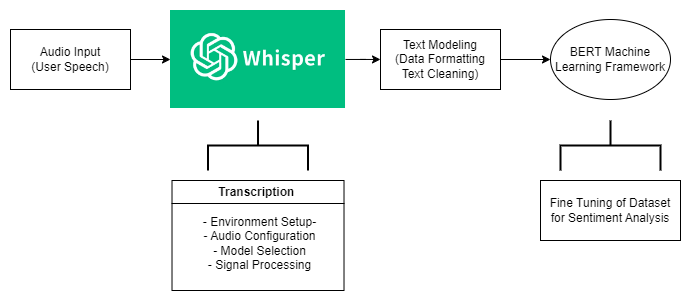
\includegraphics[width=\linewidth]{ICLR 2025 Template/nlp.drawio.png}

\newpage
\section{Experiment setup and evaluation}
For this project, we utilize the GoEmotions dataset, which includes 58,000 Reddit comments labeled with 27 emotion categories, to fine-tune our sentiment analysis models, BERT. Additionally, we use diverse speech samples from various speakers, encompassing different accents, speaking styles, and background noises, to ensure the robustness of our speech recognition component.

Our evaluation protocol involves assessing the speech recognition accuracy by calculating the Word Error Rate (WER) of OpenAI Whisper API against ground truth transcripts. For sentiment classification, we measure the performance of BERT using accuracy, precision, recall, and F1-score, along with confusion matrices to evaluate the correct classification of each emotion category. To ensure real-time functionality, we also evaluate the system’s latency and throughput, measuring the time from audio input to sentiment output and the ability to handle multiple conversations simultaneously.

The experimental procedure begins with fine-tuning the sentiment models on the GoEmotions dataset, followed by integrating the speech recognition APIs into the pipeline. We conduct initial tests with the collected speech samples to verify transcription accuracy and then evaluate the sentiment analysis performance using the defined metrics. Based on the results, we iteratively refine the models and pipeline to address any issues with transcription errors or classification inaccuracies. Finally, we perform a comprehensive evaluation to validate the system’s effectiveness in accurately and efficiently detecting emotions in real-time conversations.



\section{Results obtained so far}
Preliminary results indicate that the BERT model, fine-tuned on the GoEmotions dataset, achieved high accuracy in emotion classification. To accommodate slight variations in parsing human speech, we aimed to perform extensive preparation for finding a practical and efficient API for ingesting and analyzing audio inputs.

Our progress has advanced to a stage where we have successfully implemented a working solution for converting human speech to text using the OpenAI Whisper API. This implementation involves several steps: first, we configured the Whisper API to ensure optimal performance for our specific use case. We chose the appropriate model size based on our needs, balancing accuracy and processing time. The API offers various configurations, including support for multiple languages, noise robustness, and options for real-time or batch processing, which we tailored to suit the characteristics of the audio inputs we expect to handle.

To facilitate the integration, we developed a pipeline that captures audio input from users, processes it through the Whisper API, and retrieves the transcribed text. We implemented error handling to manage issues such as background noise and interruptions in speech, enhancing the reliability of the transcription. With the Whisper API's ability to perform well even in challenging audio environments, we were able to achieve high transcription accuracy, significantly reducing the manual effort required for text conversion.

Having established this critical milestone, our next direction involves training the transcribed text for sentiment analysis. We plan to employ various machine learning techniques and sentiment classification models, leveraging existing datasets and possibly fine-tuning pre-trained models on our specific data. This step will enhance our system's capability to understand and interpret the emotional nuances present in the spoken content. By providing deeper insights into the emotional context of conversations, we aim to improve the overall functionality and effectiveness of our project, ultimately leading to a more intuitive human-computer interaction experience




\section{Challenges and solutions}
One significant challenge we have encountered in our project is ensuring the accuracy of speech transcription across diverse audio inputs. Variations in accents, speaking speeds, and background noise can lead to transcription errors, which subsequently affect the reliability of sentiment analysis. To address this, we are incorporating a diverse set of speech samples during the training phase to make the speech recognition models more robust. Additionally, we plan to implement noise reduction and audio normalization techniques during the pre-processing stage to enhance transcription quality.

Another difficulty lies in effectively fine-tuning the sentiment analysis models, BERT, on the GoEmotions dataset to accurately capture subtle emotional nuances. The complexity of emotions and their overlapping characteristics can make precise classification challenging. To overcome this, we are experimenting with various fine-tuning strategies, such as adjusting learning rates and using cross-validation techniques to optimize model performance. Furthermore, we are exploring the use of data augmentation methods to increase the diversity of training samples, thereby improving the models' ability to distinguish between closely related emotions.

\section{Related Work}

Existing studies on OpenAI Whisper have shown highly appealing capabilities in optimizing the transcription process. Many of these existing implementations showcase unique ways of leveraging OpenAI's Whisper AI for the transcription of audio files. For example, Whisper AI can be used in mental health research, highlighting its unique capabilities in streamlining what has traditionally been a labor-intensive process. By integrating Whisper AI, researchers can optimize transcription efficiency while minimizing errors, a significant improvement over conventional methods. What sets this article apart is its detailed, step-by-step approach to implementing a transcription pipeline specifically tailored for psychology, psychiatry, and neuroscience research (Spiller et. al, 2023). It not only covers the technical setup—such as recording, preprocessing, and post-processing audio data—but also includes practical examples in a Python environment, enabling researchers to easily replicate the process. Additionally, the discussion of privacy and Institutional Review Board (IRB) considerations underscores the ethical dimensions of using AI in sensitive research areas, making this tutorial particularly relevant for researchers seeking to incorporate advanced technology while adhering to ethical standards.




In the realm of speech recognition, Yoon et al. (2023) evaluated various speech-to-text APIs, including OpenAI Whisper, for their effectiveness in transcribing emotional speech. Their research, titled "LI-TTA: Language Informed Test-Time Adaptation for Automatic Speech Recognition," highlighted Whisper’s superior performance in handling diverse accents and emotional intonations, which aligns with our decision to adopt Whisper for speech transcription. By leveraging Whisper, we benefit from its high accuracy and robustness in transcribing varied speech patterns, ensuring reliable input for our sentiment analysis.



Additionally, Li et al. (2023) presented an innovative approach in "Improving Speech Recognition Performance in Noisy Environments by Enhancing Lip Reading Accuracy." They proposed integrating lip-reading capabilities with speech recognition to bolster performance in noisy settings. By constructing a one-to-many mapping model between lip movements and speech, and employing cross-modal fusion techniques, their method significantly reduced the Word Error Rate (WER) in challenging acoustic environments. This aligns with our project's focus on leveraging advanced speech recognition (Whisper) and sentiment analysis (BERT) to improve emotion detection accuracy. Incorporating visual information, as demonstrated by Li et al., could further enhance our system's ability to accurately interpret emotions from speech, especially in noisy conditions.



\newpage
Citations: \\ \\ 
\begin{hangparas}{15pt}{1}  % Adjust the indent (15pt) and line spacing (1) as needed
Spiller, T. R., Rabe, F., Ben-Zion, Z., Korem, N., Burrer, A., Homan, P., Duek, O. (2023, April 27). Efficient and accurate transcription in mental health research - A tutorial on using Whisper AI for audio file transcription. https://doi.org/10.31219/osf.io/9fue8
\end{hangparas}

\begin{itemize}
    \item \url{https://arxiv.org/html/2407.21315v1}
    \item \url{https://arxiv.org/html/2406.18088v2}
    \item \url{https://deepgram.com/learn/ai-speech-audio-intelligence-sentiment-analysis-intent-recognition-topic-detection-api}
    \item \url{https://www.observe.ai/blog/voice-analytics}
    \item \url{https://research.aimultiple.com/audio-sentiment-analysis/}
    \item \url{https://www.assemblyai.com/products/speech-understanding}
    \item \url{https://www.reddit.com/r/singularity/comments/1bpailv/you_guys_have_to_try_this_new_empathy_llm_demo_it/}
    \item \url{https://ieeexplore.ieee.org/stamp/stamp.jsp?arnumber=8852707}
    \item \url{https://www.isca-archive.org/interspeech_2021/zhou21b_interspeech.pdf}
    \item \url{https://arxiv.org/abs/2408.05769}
    \item \url{https://www.mdpi.com/1424-8220/23/4/2053}
\end{itemize}



\end{document}
